\documentclass[11pt,class=report,crop=false]{standalone}
\usepackage[screen]{../python}



\begin{document}

\definecolor{coul_prive}{rgb}{0.93,0.26,0}
\definecolor{coul_public}{rgb}{0.06,0.63,0}

\newcommand{\prive}[1]{\relax\ifmmode{\color{coul_prive} #1}\else{\bf\color{coul_prive} #1}\fi}
\newcommand{\public}[1]{\relax\ifmmode{\color{coul_public} #1}\else{\bf\color{coul_public} #1}\fi}


%====================================================================
\chapitre{Arithmétique}
%====================================================================

\insertvideo{qPgqcSA8dzc}{partie 12.1. Éléments d'arithmétique}

\insertvideo{gBHNuFq5PpI}{partie 12.2. Cryptographie RSA}



\objectifs{La sécurité des communications sur internet est basée sur l'arithmétique et en particulier sur le système de cryptographie RSA qui repose sur la difficulté de factoriser de très grands entiers avec un ordinateur classique. Nous présentons dans ce chapitre les notions essentielles d'arithmétique afin de comprendre plus tard l'algorithme de Shor qui permet de factoriser rapidement un entier à l'aide d'un ordinateur quantique.}


%%%%%%%%%%%%%%%%%%%%%%%%%%%%%%%%%%%%%%%%%%%%%%%%%%%%%%%%%%%%%%%%%%%%%
\section{Division et pgcd}

%--------------------------------------------------------------------
\subsection{Divisibilité}

\begin{definition}
Soient $a,b \in \Zz$ avec $b$ non nul. On dit que $b$ \defi{divise} $a$ s'il existe un entier $k\in\Zz$ tel que \myboxinline{$a=kb$}.
\end{definition}
On note alors $b | a$. On dit aussi que $a$ est divisible par $b$ ou encore que $b$ est un diviseur de $a$.

Par exemple :
\begin{itemize}
  \item $3 | 12$ (\og{}$3$ divise $12$\fg{} ou bien \og{}$12$ est divisible par $3$\fg{}).
  \item Plus généralement les diviseurs positifs de $12$ sont $1$, $2$, $3$, $4$, $6$, $12$.
  \item Quel que soit $b\in \Zz$, non nul, on a $b | 0$. 
\end{itemize}

%--------------------------------------------------------------------
\subsection{Division euclidienne}

La \defi{division euclidienne}\index{division euclidienne} permet de généraliser la notion de divisibilité.

Soient $a\in \Zz$ et $b\in \Nn\setminus \{0\}$.
Il existe des entiers $q,r \in \Zz$, uniques, tels que
\mybox{$a=bq+r \qquad \text{ et } \qquad  0 \le r < b$}

\begin{itemize}
  \item L'entier $q$ est le \defi{quotient} et $r$ est le \defi{reste}. 
  \item Exemple : $a=101$, $b=7$ alors $q=14$ et $r=3$ car $101 = 7 \times 14 +3$.
  \item Le reste est nul si et seulement si $b$ divise $a$.
  \item On note aussi (de façon un peu abusive) $r = a \pmod{b}$. 
  \item Avec \Python{} on calcule le quotient par \ci{q = a//b} (à noter la double barre de division) et le reste \ci{r = a \% b}.  
\end{itemize}

%--------------------------------------------------------------------
\subsection{Pgcd}

Soient $a,b \in \Zz$ (non tous les deux nuls).
Le \defi{pgcd}\index{pgcd} de $a$ et $b$ est le plus grand entier qui divise à la fois $a$ et $b$.

Par exemple avec $a = 42$ et $b=24$, les diviseurs positifs communs à $a$ et $b$ sont
$\{1,2,3,4,6\}$, donc $\pgcd(42,24)=6$.

%--------------------------------------------------------------------
\subsection{Nombres premiers entre eux}

Les entiers $a$ et $b$ sont \defi{premiers entre eux} si leur pgcd vaut $1$.

Par exemple $a=20$ et $b=33$ sont premiers entre eux, car le seul diviseur positif de ces deux entiers est $1$.

Autre exemple : deux entiers consécutifs sont toujours premiers entre eux. Preuve : si $d>0$ divise $a$ et $a+1$ alors $d$ divise $(a+1) - a$, donc $d$ divise $1$, donc $d$ égal $1$.

%--------------------------------------------------------------------
\subsection{Théorème de Bézout}

\begin{theoreme}[Théorème de Bézout]
\index{theoreme de Bezout@théorème de Bézout}
Soient $a,b$ des entiers non nuls. Il existe
des entiers $u,v \in \Zz$ tels que
\mybox{$au+bv=\pgcd(a,b)$}
\end{theoreme}

On a même une équivalence lorsque les entiers sont premiers entre eux :
\begin{corollaire}
Soient $a, b$ deux entiers non nuls. $a$ et $b$ sont premiers entre eux
si et seulement si il existe $u,v \in \Zz$ tels que
\mybox{$au+bv=1$}
\end{corollaire}

Exemples :
\begin{itemize}
  \item $a = 42$ et $b=24$. On a vu $\pgcd(42,24)=6$. Avec $u=-1$ et $v=2$, on obtient
$42 \times (-1) + 24 \times 2 = 6$.
  \item $a=20$ et $b=33$. On a vu $\pgcd(20,33)=1$.  Avec $u=5$ et $v=-3$, on obtient
$20 \times 5+ 33 \times (-3) = 1$.
\end{itemize}

%--------------------------------------------------------------------
\subsection{Algorithme d'Euclide}

\index{algorithme d'Euclide}

L'algorithme d'Euclide est une méthode efficace pour calculer le pgcd et sa version étendue permet de trouver des coefficients $u,v$ du théorème de Bézout.

Soient $a,b \in \Nn^*$. Considérons la division euclidienne $a=bq+r$, où $r$ est le reste. Alors
\mybox{$\pgcd(a,b)=\pgcd(b,r)$}

Pour en faire un algorithme on calcule des divisions euclidiennes successives. Le pgcd sera le dernier reste
non nul car on sait que $\pgcd(a,0)=a$.

\begin{exemple}
Calculons le pgcd $d$ de $a=11\,466$ et $b=1656$.
\begin{itemize}
 \item Division euclidienne de $a$ par $b$ : $11\,466 = 6 \times 1656 + 1530$, donc le reste est $r_1=1530$.
On utilise alors $d=\pgcd(a,b)=\pgcd(b,r_1)$, donc $\pgcd(11\,466,1656)=\pgcd(1656,1530)$.
 \item Division euclidienne de $b=1656$ par $r_1=1530$ : $1656 = 1 \times 1530 + 126$, donc le reste est $r_2=126$.
Notre pgcd $d$ vaut maintenant $\pgcd(1530,126)$.
 \item Division euclidienne de $1530$ par $126$ : $1530 = 12 \times 126 + 18$, donc le reste est $r_3=18$
et $d=\pgcd(126,18)$.
 \item Division euclidienne de $128$ par $18$: $126 = 7 \times 18 + 0$, donc le reste est nul. Or $\pgcd(18,0)=18$.
 \item Le pgcd est le dernier reste non nul, ainsi $\pgcd(11\,466,1656) = 18$.
\end{itemize}

\end{exemple}

L'algorithme d'Euclide est l'un des plus anciens algorithmes mais il est cependant très efficace !
Le nombre d'étapes dans l'algorithme est assez faible : si $a$ et $b$ s'écrivent (en base $10$) avec moins de $n$ chiffres, alors il y a au plus $5n$ étapes dans l'algorithme d'Euclide. Donc par exemple, avec des entiers à $100$ chiffres, il y a au plus $500$ étapes. 
% En plus à chaque étape, on a juste besoin de calculer le reste d'une division euclidienne (mais pas le quotient).

%--------------------------------------------------------------------
\subsection{Lemme de Gauss}

\begin{proposition}[Lemme de Gauss]
\index{lemme de Gauss}
Soient $a,b,c \in \Zz$ (avec $a$ non nul).
\mybox{Si \ \ $a | bc$ \ \  et \ \  $\pgcd(a,b)=1$ \ \  alors \ \  $a|c$}
\end{proposition}

Exemple : si un entier $a$ divise $(a+1)c$ alors $a|c$ (c'est le lemme de Gauss, sachant qu'on a toujours $\pgcd(a,a+1)=1$).

Attention aux hypothèses : $6$ divise $4 \times 9$, mais $6$ ne divise ni $4$  ni $9$. Cela ne contredit pas le lemme de Gauss car $6$ n'est premier ni avec $4$, ni avec $9$.

La preuve découle du théorème de Bézout : comme par hypothèse $\pgcd(a,b)=1$,
il existe $u,v\in \Zz$ tels que $au+bv=1$. On multiplie cette égalité par $c$ pour obtenir
$acu + bcv = c$. Mais $a|acu$ et par hypothèse $a|bcv$ donc
$a$ divise $acu+bcv=c$.

%%%%%%%%%%%%%%%%%%%%%%%%%%%%%%%%%%%%%%%%%%%%%%%%%%%%%%%%%%%%%%%%%%%%%
\section{Nombres premiers}

%--------------------------------------------------------------------
\subsection{Définition}

\begin{definition}
Un \defi{nombre premier}\index{nombre premier} $p$ est un entier supérieur ou égal à $2$ dont les seuls diviseurs
positifs sont $1$ et $p$.
\end{definition}

Exemples.
\begin{itemize}
  \item $2,3,5,7,11,13,\ldots$ sont des nombres premiers.
  \item Un théorème d'Euclide nous dit qu'il y a une infinité de nombres premiers.
%  \item $6 = 2 \times 3$ n'est pas un nombre premier.
  \item Par définition, $1$ n'est pas un nombre premier.
\end{itemize}


%--------------------------------------------------------------------
\subsection{Décomposition en facteurs premiers}

\begin{theoreme}
Tout entier $n\ge2$ se décompose en produit de facteurs premiers :
$$n = p_1^{\alpha_1} \times p_2^{\alpha_2} \times \cdots \times p_r^{\alpha_r}$$
où les $p_i$ sont des nombres premiers, et les exposants $\alpha_i\ge1$ sont des entiers.
De plus, cette décomposition est unique (à l'ordre des facteurs près).
\end{theoreme}

%--------------------------------------------------------------------
\subsection{Petit théorème de Fermat}


\begin{theoreme}[Petit théorème de Fermat]
\index{theoreme de Fermat@(petit) théorème de Fermat}
Si $p$ est un nombre premier ne divisant pas $a$ alors
\mybox{$a^{p-1} \equiv 1 \pmod p$}
\end{theoreme}

Une variante : pour $a$ un entier quelconque et $p$ un nombre premier : 
\mybox{$a^{p} \equiv a \pmod p$}

Nous reviendrons sur les congruences dans la section suivante.


%--------------------------------------------------------------------
\subsection{Algorithmes et nombres premiers}

Nous allons discuter de plusieurs algorithmes qui permettent de décider si un entier $n$ donné est un nombre premier ou pas.

\textbf{Tester les diviseurs un par un.}
On teste si $d$ divise $n$ pour $d=2$, $d=3$, $d=4$,\ldots{} Cela se fait par un calcul de division euclidienne. Si on obtient un diviseur strictement inférieur à $n$, alors $n$ n'est pas premier. Si on ne trouve pas de diviseur alors $n$ est premier.

Améliorations possibles : on peut tester $d=2$, et ensuite ne tester que des entiers $d$ impairs ;
on peut aussi limiter la recherche des diviseurs à ceux vérifiant $d \le \sqrt{n}$ (critère de Napoléon).

\bigskip
\textbf{Crible d'Ératosthène.}
On peut aussi dresser une longue liste de nombres premiers, au delà de l'entier $n$. 
L'avantage est qu'il suffit alors de vérifier si l'entier $n$ est dans la liste pour savoir s'il est premier. Mais le crible est une méthode lente et ne permet pas d'obtenir de très grands nombres premiers.

\bigskip
\textbf{Test probabiliste de Fermat.}
Le petit théorème de Fermat nous dit que si $p$ est un nombre premier et $a$ est un entier avec $1 \le a < p$ alors $a^{p-1} \equiv 1 \pmod p$.

Pour tester si un entier $n$ est premier, on fixe un entier $1 < a < n$, on calcule $a^{n-1} \pmod n$ (c'est très facile grâce à l'exponentiation rapide, voir plus loin). 
\begin{itemize}
  \item Si $a^{n-1} \not\equiv 1 \pmod{n}$ alors on est sûr que $n$ n'est pas un nombre premier.
  \item Si $a^{n-1} \equiv 1 \pmod{n}$ alors on dit que $n$ valide le test de Fermat pour l'entier $a$ et qu'il est probablement premier. Cependant il existe des exceptions : certains entiers valident le test de Fermat mais ne sont pas des nombres premiers. Par exemple parmi tous les entiers $n \le 1\,000\,000$, tous ceux qui passent le test de Fermat à la fois pour $a=2$, $a=3$, $a=5$ et $a=7$ sont des nombres premiers (il y en a $78\,498$) à l'exceptions de $19$ entiers (le premier de la liste est $n=29\,341=13\times37\times61$).
\end{itemize}

Le test de Fermat permet de produire des entiers très grands qui sont probablement des nombres premiers : on choisit un entier impair $n$ au hasard, on effectue un test de Fermat, si le test est concluant alors $n$ est probablement un nombre premier, sinon on essaie l'entier $n+2$\ldots

\bigskip
\textbf{Algorithmes modernes.}
Une amélioration du test de Fermat est l'algorithme de Miller-Rabin.
Par ailleurs, il a été récemment démontré par Agrawal--Kayal--Saxena que le test de primalité peut être effectué en temps polynomial (algorithme AKS). Même si dans la pratique l'algorithme n'est pas très utile, c'est une grande avancée théorique. L'algorithme est basé sur le fait que si $p$ est un nombre premier alors on a l'égalité polynomiale : $(X+1)^p \equiv X^p+1 \pmod p$.

%--------------------------------------------------------------------
\subsection{Algorithmes et factorisation}

Tester si un entier est premier ou donner sa factorisation sont au final deux problèmes distincts.
On a vu, grâce au petit théorème de Fermat, qu'on peut décider qu'un entier n'est pas premier sans lui avoir trouvé de facteur.
Le problème de factoriser un entier $n$, ou au moins de trouver un facteur non trivial, est donc plus difficile.

\bigskip
\textbf{Tester les diviseurs un par un.}
Comme auparavant on peut tester les diviseurs un par un jusqu'à $\sqrt{n}$, la complexité est en $O(\sqrt{n})$. On peut bien sûr ne tester que les diviseurs premiers (ce qui est plus rapide) mais cela demande au préalable d'avoir une liste des premiers nombres premiers (ce qui est long).
C'est donc une méthode efficace uniquement pour trouver les petits diviseurs.

\bigskip
\textbf{Facteurs de Fermat.}
On peut essayer d'exprimer $n$ comme différence de deux carrés, on obtient alors une factorisation. En effet, si c'est le cas :
$$n= a^2-b^2 = (a-b)(a+b).$$
Réciproquement tout entier impair non premier est la différence de deux carrés.
En effet, si $n = cd$ alors $n = \left(\frac{c+d}{2}\right)^2 - \left(\frac{c-d}{2}\right)^2.$
Cela fournit un algorithme de recherche d'un facteur de $n$ : prendre un entier $a$ (généralement proche de $\sqrt{n}$), calculer si $b'=n-a^2$ est un carré de la forme $b^2$, si c'est le cas, on obtient une factorisation $(a-b)(a+b)$, sinon on recommence avec $a+1$. 
C'est une méthode efficace si les facteurs premiers sont grands, donc cette méthode est complémentaire de la précédente.

\bigskip
\textbf{Algorithmes modernes.}

Aucun algorithme connu n'a de complexité polynomiale. Plus précisément, on ne connaît pas d'algorithme de factorisation ayant une complexité polynomiale, mais on ne sait pas non plus prouver qu'un tel algorithme n'existe pas.

Le meilleur algorithme connu pour factoriser des grands entiers est l'algorithme GNFS (pour \emph{General Number Field Sieve}), sa complexité est environ $O(n^{\frac13})$ (c'est donc une complexité exponentielle par rapport à la taille de $n$ qui est d'ordre $\ln(n)$).

 

%%%%%%%%%%%%%%%%%%%%%%%%%%%%%%%%%%%%%%%%%%%%%%%%%%%%%%%%%%%%%%%%%%%%%
\section{Congruence modulo $n$}

\index{congruence}
\index{modulo}

%--------------------------------------------------------------------
\subsection{Modulo $n$}

\begin{definition}
Soit $n\ge1$ un entier. On dit $a \equiv b \pmod n$ s'il existe $k\in\Zz$ tel que $a=kn+b$, autrement dit si $b-a$ est divisible par $n$.
On dira \defi{$a$ est congru à $b$ modulo $n$}.
\end{definition}

\begin{proposition}
Si $a \equiv b \pmod n$ et $a' \equiv b' \pmod n$ alors :
$$a+a' \equiv b+b' \pmod n \qquad \text{ et } \qquad a \cdot a' \equiv b \cdot b' \pmod n.$$
De plus $a^k \equiv b^k \pmod n$, quel que soit $k \in \Nn$.
\end{proposition}

\emph{Exemples.}
\begin{itemize}
  \item $33 \equiv 3 \pmod{15}$ car $33 = 2 \times 15 + 3$.
  \item $1789 = 105 \times 17 + 4$ donc $1789 \equiv 4 \pmod{17}$, mais aussi $1789 = 104 \times 17 + 21$ et $1789 \equiv 21 \pmod{17}$.
  \item Un entier $a$ est pair si et seulement si $a \equiv 0 \pmod 2$.
  \item Par conséquent si $a$ est impair alors $a^k$ est impair. En effet $a$ impair, implique $a \equiv 1 \pmod 2$,
donc $a^k \equiv 1^k \equiv 1 \pmod 2$, donc $a^k$ est impair.
\end{itemize}

%--------------------------------------------------------------------
\subsection{Inverse modulo $n$}

\begin{definition}
Soit $n\ge1$ un entier. On dit que $a$ est \defi{inversible} modulo $n$, s'il existe $b\in\Zz$ tel que $a \cdot b \equiv 1 \pmod n$.
On dit alors que $b$ est l'inverse de $a$ modulo $n$.
\end{definition}

\emph{Exemples.}
\begin{itemize}
  \item Avec $n=15$, $a=2$ est inversible modulo $15$, car avec $b=8$ on $a \cdot b = 2 \times 8 = 16 \equiv 1 \pmod{15}$.
  \item Avec $n=15$, $a=7$ est inversible modulo $15$, car avec $b=13$ on $a \cdot b = 7 \times 13 = 91 \equiv 1 \pmod{15}$.    
  \item Avec $n=15$, $a=3$ n'est pas inversible.
\end{itemize}

\begin{proposition}
$a$ est inversible modulo $n$ si et seulement si $\pgcd(a,n)=1$.
\end{proposition}

\begin{proof}
\begin{align*}
    \pgcd(a,n)=1 \iff& \exists u,v \in \Zz \quad au+nv = 1 \qquad \text{(par le théorème de Bézout)} \\
\iff& \exists u,v \in \Zz \quad au = 1 - nv \\
\iff& \exists u \in \Zz \quad au \equiv 1 \pmod{n} \\
\iff& \text{$a$ est inversible modulo $n$.} \\
\end{align*}
\end{proof}

La preuve justifie que l'on peut trouver l'inverse de $a$ modulo $n$ à l'aide des coefficients de Bézout $u$, $v$. Ces coefficients se calculent à l'aide de l'algorithme d'Euclide étendu.



%--------------------------------------------------------------------
\subsection{Groupes}

\index{groupe!zn@$\Zz/n\Zz$}

Pour être un peu plus théorique, on définit :
\begin{itemize}
  \item $\big( \Zz/n\Zz, +\big)$ le groupe additif des entiers modulo $n$. C'est un groupe commutatif ($a+b \equiv b+a \pmod n$), ayant $n$ éléments.
L'élément neutre pour l'addition est $0$, l'inverse d'un élément $a$ est $-a$.
  \item $\big( (\Zz/n\Zz)^*, \times \big)$ le groupe des inversibles modulo $n$. C'est un groupe multiplicatif, commutatif ($a\times b \equiv b\times a \pmod n$).
Son élément neutre est $1$, l'inverse d'un élément $a$ est son inverse modulo $n$, noté $b$, tel que $ab \equiv 1 \pmod n$.
Le groupe $(\Zz/n\Zz)^*$ possède $\varphi(n)$ éléments (où $\varphi(n)$ est défini juste après).
\end{itemize}



%--------------------------------------------------------------------
\subsection{Indicatrice d'Euler}

\begin{definition}
Soit $n\ge1$. L'\defi{indicatrice d'Euler}\index{indicatrice d'Euler} $\varphi(n)$ est le nombre d'entiers $a$ 
premiers avec $n$, tels que $1 \le a \le n$.
\end{definition}

Une conséquence immédiate est que $\varphi(n)$ est le nombre d'éléments inversibles modulo $n$ : $\varphi(n) = \operatorname{Card} (\Zz/n\Zz)^*$.

Exemples.
\begin{itemize}
  \item Soit $n=15$. Les entiers $a$ premiers avec $15$ sont 
$\{1,2,4,7,8,11,13,14\}$, donc $\varphi(n) = 8$.
  \item Si $p$ est nombre premier alors $\varphi(p)=p-1$ car tout entier $a$, avec $1 \le a < p$, est premier avec $p$.
\end{itemize}

La proposition suivante permet de calculer $\varphi(n)$ à partir de la décomposition de $n$ en facteurs premiers.

\begin{proposition}
\sauteligne
\begin{itemize}
  \item Si $n=pq$ (avec $p,q$ deux nombres premiers distincts) alors 
$\varphi(n) = (p-1)(q-1)$.
  \item S $n = p^k$ (avec $k\ge1$) alors $\varphi(n) = p^k-p^{k-1}$.
  \item Formule générale. Si $n=p_1^{\alpha_1}\cdots p_\ell^{\alpha_\ell}$ alors
$$\varphi(n) = n \prod_{i=1}^\ell \left( 1 - \frac{1}{p_i} \right).$$
\end{itemize}
\end{proposition}

\begin{proof}~
\begin{itemize}
  \item Si $n=pq$ alors les entiers $a$ qui \emph{ne sont pas} premiers avec $n$ sont les $p,2p,3p,\ldots,(q-1)p$ et les $q,2q,\ldots,(p-1)q$ et $pq$.
Il y a en a donc $(q-1) + (p-1) + 1= p+q-1$. Les autres sont premiers avec $n$ et sont au nombre de $pq - (p+q-1) = (p-1)(q-1)$.
  \item Si $n = p^k$ alors les entiers qui ne sont pas premiers avec $n$ sont les multiples de $p$ de la forme $\alpha p$ avec $1\le \alpha \le p^{k-1}$. Il y en a donc $p^{k-1}$.
  \item Nous admettons la formule générale qui se prouve par récurrence à partir de la formule $\varphi(ab) = \varphi(a)\cdot \varphi(b)$ lorsque $a$ et $b$ sont premiers entre eux.
\end{itemize}
\end{proof}


%--------------------------------------------------------------------
\subsection{Théorème d'Euler}

Le théorème d'Euler est une version généralisée du petit théorème de Fermat.
\begin{theoreme}[Théorème d'Euler]
\index{theoreme d'Euler@théorème d'Euler}
Si $a$ et $n$ sont premiers entre eux alors :
\mybox{$a^{\varphi(n)} \equiv 1 \pmod{n}$}
\end{theoreme}

On pourrait déduire ce résultat du théorème de Lagrange appliqué au groupe fini $(\Zz/n\Zz)^*$ de cardinal $\varphi(n)$.
Nous allons en donner une autre démonstration.
\begin{proof}
Fixons $n$ et fixons $a$ premier avec $n$. 
Notons $\mathcal{A} = \{ a_1,a_2,\ldots,a_{\varphi(n)} \}$ l'ensemble des entiers inférieurs à $n$ et premiers avec $n$ (notre entier $a$ est l'un de ces éléments et en fait $\mathcal{A}=(\Zz/n\Zz)^*$).
Considérons l'application $f : \mathcal{A} \to \mathcal{A}$, définie par $f(a_i) = a \cdot a_i \pmod n$. Comme $a$ est inversible modulo $n$, alors $f$ est bijective (sa bijection réciproque est $f^{-1}(a_i) = b \cdot a_i \pmod n$ où $b$ est l'inverse de $a$ modulo $n$).
Ainsi $\mathcal{A'} = \{a\cdot a_1,a\cdot a_2,\ldots,a\cdot a_{\varphi(n)}\}$ contient les mêmes termes que notre ensemble $\mathcal{A} = \{ a_1,\ldots,a_{\varphi(n)} \}$ (mais les éléments sont permutés) : $\mathcal{A}'=\mathcal{A}$. Comme ces ensembles sont égaux, alors le produit des éléments de $\mathcal{A}'$ est égal au produit des éléments de $\mathcal{A}$ :
$$\prod_{i=1}^{\varphi(n)} (a \cdot a_i) \equiv \prod_{i=1}^{\varphi(n)} a_i \pmod n$$
donc $$a^{\varphi(n)} \prod_{i=1}^{\varphi(n)} a_i \equiv \prod_{i=1}^{\varphi(n)} a_i \pmod n,$$ et comme les $a_i$ sont inversibles modulo $n$, alors 
$a^{\varphi(n)} \equiv 1 \pmod n$.
\end{proof}

%--------------------------------------------------------------------
\subsection{Exponentiation}

Fixons $n\ge1$ et $a \in \Zz$. Il s'agit de calculer $a^k \pmod n$, pour un entier $k\ge0$.

\bigskip
\textbf{Exponentiation classique.}
Si on a besoin de connaître tous les $a^k \pmod n$ pour $k=1,2,3,\ldots$ alors on les calcule successivement en utilisant la relation $a^{k+1} = a^k \cdot a$.

\begin{exemple}
Calcul des $2^k  \pmod {25}$.
$$
\setlength{\arraycolsep}{20pt}
\begin{array}{ll}
2^0 \equiv 1 \pmod{25} & 2^5 \equiv 2 \times 16 \equiv 7  \pmod{25}\\
2^1 \equiv 2 \pmod{25} & 2^6 \equiv 2 \times 7 \equiv 14 \pmod{25} \\
2^2 \equiv 2\times 2 \equiv 4 \pmod{25} &2^7 \equiv 2 \times 14 \equiv 28 \equiv 3  \pmod{25}\\
2^3 \equiv 2 \times 4 \equiv 8 \pmod{25} &   2^8 \equiv 2 \times 3 \equiv 6 \pmod{25}\\
2^4 \equiv 2 \times 8 \equiv 16 \pmod{25} & \cdots \\
\end{array}$$
Noter que chaque calcul est une simple multiplication par $a$ du résultat précédent et qu'on réduit immédiatement modulo $n$ afin que les entiers en jeu restent de petite taille.
\end{exemple}

\bigskip

\textbf{Exponentiation rapide.}
\index{exponentiation rapide}
Si on a besoin de connaître un seul $a^k \pmod n$, alors on n'est pas obligé de calculer toutes les puissances précédentes, mais seulement celles dont l'exposant $k$ est une puissance de $2$.

\begin{exemple}
On souhaite calculer $3^{21} \pmod{31}$.
\begin{itemize}
  \item On décompose l'exposant $21$ en base $2$ : $21 = 16 + 4 + 1$.
  \item On calcule successivement $3^1$, $3^2$, $3^4$, $3^8$,\ldots{} en utilisant que $3^{2k} = (3^k)^2$. De plus tous les calculs se font modulo $n=31$.
$$\begin{array}{l}
3^1 \equiv 3 \pmod{31} \\
3^2 \equiv 9 \pmod{31} \\
3^4 \equiv (3^2)^2 \equiv 9^2 \equiv 81 \equiv 19 \pmod{31} \\
3^8 \equiv (3^4)^2 \equiv 19^2 \equiv 361 \equiv 20 \pmod{31} \\
3^{16} \equiv (3^8)^2 \equiv 20^2 \equiv 400 \equiv 28 \pmod{31} \\
\end{array}$$

  \item On combine les résultats :
$$3^{21} = 3^{16+4+1} = 3^{16} \times 3^4 \times 3^1 
\equiv 28 \times 19 \times 3 \equiv 1596 \equiv 15 \pmod{31}.$$ 

\end{itemize}
\end{exemple}


%%%%%%%%%%%%%%%%%%%%%%%%%%%%%%%%%%%%%%%%%%%%%%%%%%%%%%%%%%%%%%%%%%%%%
\section{Cryptographie RSA}

\index{chiffrement!RSA}

%-------------------------------------------------------
\subsection{Chiffrement à clé secrète}

Jusqu'à récemment pour que Bob envoie un message à Alice, sans que personne ne puisse prendre connaissance du contenu, on utilisait un \defi{chiffrement à clé secrète}. Une méthode (très basique) consiste par exemple à décaler chaque lettre d'un certain rang $C$. Par exemple si $C=3$, Bob chiffre son message \prive{BAC} en \public{EDF}. Alice peut facilement déchiffrer le message si elle connaît la clé $C$.

On représente ce protocole ainsi : Bob dépose son message dans un coffre fort pour Alice,
Alice et Bob étant les seuls à posséder la clé du coffre.
\begin{center}
\begin{tikzpicture}
  \node at (-0.7,0){
  \includegraphics[height=3cm]{figures/coffre.png}
  };
  \node at (-3,-3) {\bf ALICE};
  \node at (-5,-1) {\bf BOB};

  \draw[->, blue, ultra thick] (-5,-0.7) to[bend left, thick]node[above, midway]{} (-1,0);
  \draw[->, blue, ultra thick] (-1.2,-0.5) to[bend right, thick]node[above, midway]{} (-3,-2.7);

\end{tikzpicture}
\end{center}


La grande difficulté est que Alice et Bob doivent d'abord se communiquer la clé.


\begin{center}
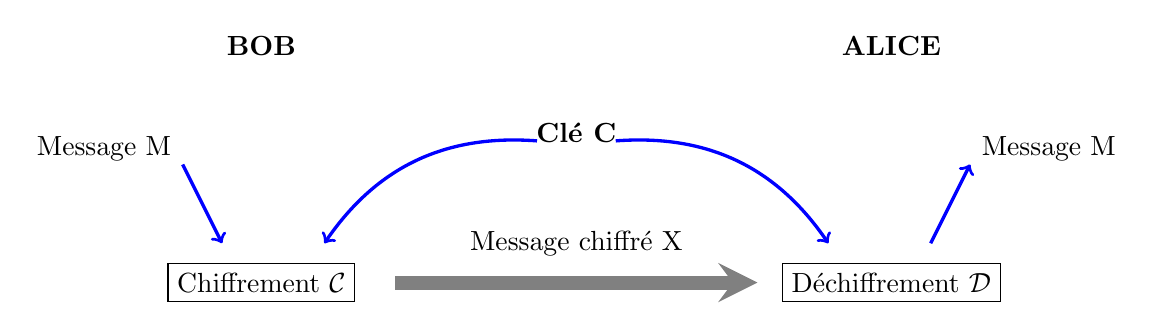
\begin{tikzpicture}

  \node at (4,3) {\bf ALICE};
  \node at (-4,3) {\bf BOB};

  \draw[line width=5pt,>=stealth,->,gray] (-2.3,0) to (2.3,0);

  \node at (-6,1.7) {\prive{Message M}};
  \node at (6,1.7) {\prive{Message M}};
  \node at (0,0.5) {\public{Message chiffré X}};
  \node at (0,1.9) {\bf Clé C};
  \draw (-4,0)node[draw]{Chiffrement \public{$\mathcal{C}$}};
  \draw (4,0)node[draw]{Déchiffrement \public{$\mathcal{D}$}};

  \draw[->, blue, very thick] (-0.5,1.8) to[bend right, thick] (-3.2,0.5);
  \draw[->, blue, very thick] (0.5,1.8) to[bend left, thick] (3.2,0.5);

  \draw[->, blue, very thick] (-5,1.5) to (-4.5,0.5);
  \draw[<-, blue, very thick] (5,1.5) to (4.5,0.5);
\end{tikzpicture}
\end{center}


%-------------------------------------------------------
\subsection{Chiffrement à clé publique}

Le chiffrement à clé publique est une petite révolution : 
n'importe qui peut envoyer un message chiffré à Alice en utilisant la clé publique d'Alice,
mais seule Alice peut déchiffrer le message à l'aide d'une clé secrète qu'elle est la seule à connaître.

De façon imagée, si Bob veut envoyer un message à Alice,
il dépose son message dans la boîte aux lettres d'Alice, seule Alice pourra ouvrir sa boîte
et consulter le message. Ici la clé publique est symbolisée par la boîte aux lettres, tout le monde peut y déposer un message, la clé qui ouvre la boîte aux lettres est la clé privée d'Alice.

\begin{center}
\begin{tikzpicture}
  \node at (-0.45,-0.56){
  \includegraphics[height=3cm]{figures/boite.png}
  };
  \node at (-3,-3) {\bf ALICE};
  \node at (-5,-1) {\bf BOB};

  \draw[->, myred, ultra thick] (-5,-0.7) to[bend left, thick]node[above, midway]{} (-1.5,-0.15);
  \draw[->, myred, ultra thick] (-2,-0.7) to[bend right, thick]node[above, midway]{} (-3,-2.7);

\end{tikzpicture}
\end{center}


Si Bob veut envoyer un message secret à Alice, le processus se décompose ainsi :
\begin{enumerate}
  \item Alice prépare une clé publique et une clé privée,
  \item Bob utilise la clé publique d'Alice pour chiffrer son message,
  \item Alice reçoit le message chiffré et le déchiffre grâce à sa clé privée.
\end{enumerate}

\begin{center}
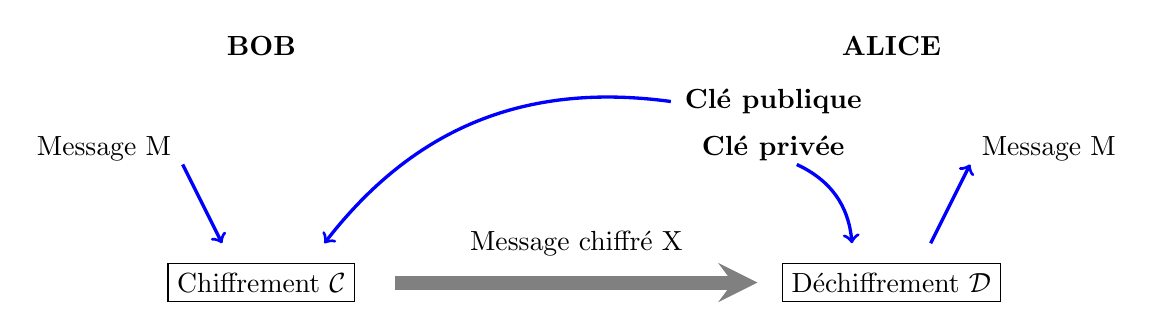
\begin{tikzpicture}

  \node at (4,3) {\bf ALICE};
  \node at (-4,3) {\bf BOB};

  \draw[line width=5pt,>=stealth,->,gray] (-2.3,0) to (2.3,0);

  \node at (-6,1.7) {\prive{Message M}};
  \node at (6,1.7) {\prive{Message M}};
  \node at (0,0.5) {\public{Message chiffré X}};
  \node at (2.5,2.3) {\bf Clé publique};
  \node at (2.5,1.7) {\bf Clé privée};
  \draw (-4,0)node[draw]{Chiffrement \public{$\mathcal{C}$}};
  \draw (4,0)node[draw]{Déchiffrement \public{$\mathcal{D}$}};

  \draw[->, blue, very thick] (1.2,2.3) to[bend right, thick] (-3.2,0.5);
  \draw[->, blue, very thick] (2.8,1.5) to[bend left, thick] (3.5,0.5);

  \draw[->, blue, very thick] (-5,1.5) to (-4.5,0.5);
  \draw[<-, blue, very thick] (5,1.5) to (4.5,0.5);
\end{tikzpicture}
\end{center}

Pour chiffrer un message, on commence par le transformer en un --ou plusieurs-- nombres.
Dans toute la suite le message que Bob envoie est un entier.

%--------------------------------------------------------------------
\subsection{Principe du chiffrement RSA}

Voici en résumé le protocole RSA.
\begin{itemize}
  \item On choisit deux nombres premiers $p$ et $q$ que l'on garde secrets et on pose $n=p\times q$. Le principe étant que même connaissant $n$ il est très difficile de retrouver $p$ et $q$.
  \item La clé secrète et la clé publique se déterminent à l'aide de l'algorithme d'Euclide
et des coefficients de Bézout.
  \item Les calculs de chiffrement se feront modulo $n$.
  \item Le déchiffrement fonctionne grâce au théorème d'Euler.
\end{itemize}

\bigskip

Et voici un schéma qui présente le chiffrement et le déchiffrement :
\begin{itemize}
\item \public{$n$}, \public{$e$} forment la clé publique d'Alice
\item \prive{$d$} est la clé privée d'Alice,
\item \prive{$m$} est le message secret que Bob souhaite transmettre à Alice,
\item \public{$x$} est le message chiffré que Bob calcule à partir de la clé publique d'Alice et qu'il lui transmet,
\item seule Alice peut retrouver \prive{$m$} par un calcul à partir de \prive{$x$} et de sa clé privée.
\end{itemize}

\begin{figure}[htbp]
    \begin{center}
      \setlength{\unitlength}{2547sp}%
      \begin{picture}(7000,2235)(2101,-3961)
        \thinlines
        \put(3301,-3961){\makebox(0,0)[cb]{Bob}}
        \put(6601,-3961){\makebox(0,0)[cb]{Alice}}
        \put(3301,-2061){\makebox(0,0)[cb]{\public{$n$}, \public{$e$}}}
        \put(2101,-3061){\makebox(0,0)[cc]{\prive{$m$}}}
        \put(3301,-2161){\vector( 0,-1){600}}
        \put(2401,-3061){\vector( 1, 0){600}}
        \put(3001,-3361){\framebox(600,600){\public{$\mathcal{C}$}}}
        \put(3601,-3061){\vector( 1, 0){2700}}
        \put(5001,-2761){\makebox(0,0)[cb]{$\public{x} \equiv \prive{m}^\public{e} \pmod {\public{n}} $}}
        \put(6601,-2061){\makebox(0,0)[cb]{\prive{$d$}}}
        \put(6301,-3361){\framebox(600,600){\public{$\mathcal{D}$}}}
        \put(6901,-3061){\vector( 1, 0){600}}
        \put(6601,-2161){\vector( 0,-1){600}}
        \put(7801,-3061){\makebox(0,0)[lc]{$\prive{m} \equiv \public{x}^\prive{d} \pmod{\public{n}}$}}
%        \put(4600,-3361){\includegraphics[height=1cm]{figures/boite.jpg}}
      \end{picture}
    \end{center}
  \end{figure}


%--------------------------------------------------------------------
\subsection{Protocole du chiffrement RSA}

%.......................................................
\subsubsection{Choix de deux nombres premiers}

Alice effectue, une fois pour toutes, les opérations suivantes (en secret) :
\begin{itemize}
  \item elle choisit deux nombres premiers distincts $\prive{p}$ et $\prive{q}$ (dans la pratique ce sont de très grands nombres, jusqu'à des centaines de chiffres),

  \item elle calcule $\public{n} = \prive{p} \times \prive{q}$,

  \item elle calcule $\varphi(\public{n}) = (\prive{p}-1) \times (\prive{q}-1)$.
\end{itemize}

Vous noterez que le calcul de $\prive{\varphi(n)}$ n'est possible que
si la décomposition de $\public{n}$ sous la forme $\prive{p}\times \prive{q}$ est connue.
D'où le caractère secret de $\prive{\varphi(n)}$ même si $\public{n}$ est connu de tous.


%.......................................................
\subsubsection{Choix d'un exposant et calcul de son inverse}

Alice continue :
\begin{itemize}
  \item elle choisit un exposant $\public{e}$ tel que $\pgcd(\public{e},\prive{\varphi(n)})=1$,

  \item elle calcule l'inverse $\prive{d}$ de $\public{e}$ modulo $\prive{\varphi(n)}$ :
  $\prive{d} \times \public{e} \equiv 1 \pmod {\prive{\varphi(n)}}$.
  Ce calcul se fait par l'algorithme d'Euclide étendu.
\end{itemize}

%.......................................................
\subsubsection{Clé publique/clé privée}

La \defi{clé publique} d'Alice est constituée des deux nombres :
\mybox{$\public{n}$ \  et \  $\public{e}$}

Et comme son nom l'indique, Alice communique sa clé publique au monde entier.

Alice garde pour elle sa \defi{clé privée} :
\mybox{\ $\prive{d}$\ }

Noter que le calcul de \prive{$d$} nécessite \prive{$\varphi(n)$}, qu'Alice est la seule à connaître.
Alice peut détruire $\prive{p}$, $\prive{q}$ et $\prive{\varphi(n)}$ qui ne sont plus utiles.
Elle ne conserve secrètement que sa clé privée.


%.......................................................
\subsubsection{Message chiffré}

Le message est un entier $\prive{m}$, tel que $0 \le \prive{m} < \public{n}$.

Bob récupère la clé publique d'Alice, $\public{n}$ et $\public{e}$,
avec laquelle il calcule :
\mybox{$\public{x} \equiv \prive{m}^\public{e} \pmod{\public{n}}$}

Il transmet ce message $\public{x}$ à Alice.

%-------------------------------------------------------
\subsubsection{Déchiffrement du message}

Alice reçoit le message $\public{x}$ chiffré par Bob, elle le déchiffre à l'aide de sa clé privée $\prive{d}$, par l'opération :
\mybox{$\prive{m} \equiv \public{x}^\prive{d} \pmod {\public{n}}$}


Nous allons prouver dans le lemme \ref{lem:dechiffre} que cette opération permet à 
Alice de retrouver le message original $\prive{m}$ de Bob.

%-------------------------------------------------------
\subsection{Exemple}

\textbf{Mise en place par Alice.}
\begin{itemize}
  \item Alice choisit $p=5$ et $q=11$, elle calcule $n=p\times q=55$.
  \item Elle calcule aussi $\varphi(n) = (p-1)(q-1) =  4\times 10 = 40$.
  \item Alice choisit par exemple l'entier $e=3$ qui est bien premier avec $\varphi(n)$.
  \item Alice calcule $d$, l'inverse de $e$ modulo $\varphi(n)$, ici elle trouve $d=27$ car $3\times 27 = 81 \equiv 1 \pmod {40}$.
  \item La clé publique d'Alice est $(n,e) = (55,3)$, sa clé privée est $d=27$.
\end{itemize}

\bigskip

\textbf{Envoi du message de Bob à Alice.}
\begin{itemize}
  \item Bob souhaite envoyer le message $m=41$ à Alice.
  \item Bob calcule $x \equiv m^e \pmod n$ à l'aide de la clé publique d'Alice.
Ici 
$$x \equiv  m^e \equiv 41^3 \equiv 68\,921 \equiv 6 \pmod{55}.$$
  \item Bob transmet $x=6$ à Alice.  
  \item Seule Alice peut déchiffrer le message à l'aide de sa clé secrète $d$, en effet
le calcul de $x^d \pmod{n}$ redonne le message original $m$.
Ici 
$$x^d \equiv 6^{27} \equiv 41 \pmod {55}.$$
Ainsi Alice obtient bien le message $m=41$.
(Pour le calcul de $6^{27} \pmod{55}$ on utilise les techniques d'exponentiation vues précédemment).
\end{itemize}


%-------------------------------------------------------
\subsection{Lemme de déchiffrement}

Le principe de déchiffrement repose sur le théorème d'Euler.

\begin{lemme}
\label{lem:dechiffre}
Soit $d$ l'inverse de $e$ modulo $\varphi(n)$.
\mybox{Si $x \equiv m^e \pmod n$ alors $m \equiv x^d \pmod n$.}
\end{lemme}

Ce lemme prouve bien que le message original $\prive{m}$ de Bob,
chiffré à l'aide de la clé publique d'Alice $(\public{e},\public{n})$ en le message $\public{x}$,
peut-être retrouvé par Alice à l'aide de sa clé secrète $\prive{d}$.

\begin{proof}~
\begin{itemize}
  \item Que $d$ soit l'inverse de $e$ modulo $\varphi(n)$ signifie
$d \cdot e \equiv 1 \pmod {\varphi(n)}$.
Autrement dit, il existe
$k \in \Zz$ tel que $d \cdot e = 1 + k \cdot \varphi(n)$.

  \item On rappelle que, par le théorème d'Euler,
  lorsque $m$ et $n$ sont premiers entre eux
  $$m^{\varphi(n)} \equiv 1 \pmod n.$$


  \item Supposons $\pgcd(m,n)=1$.

  Notons $x \equiv m^e \pmod n$ et calculons $x^d$ :
$$x^d \equiv (m^e)^d
      \equiv m^{e\cdot d}
      \equiv m^{1+k \cdot \varphi(n)}
      \equiv m \cdot m^{k \cdot \varphi(n)}
      \equiv m \cdot (m^{\varphi(n)})^k
      \equiv m \cdot (1)^k
      \equiv m \pmod {n}.$$

 \item On admet que si $m$ et $n$ ne sont pas premiers entre eux, le résultat reste vrai (il faut adapter les arguments précédents).
\end{itemize}

\end{proof}

\bigskip
\bigskip

\emph{Note.} Certains passages de ce chapitre sont extraits du chapitre \og{}Arithmétique\fg{} du livre \og{}Algèbre\fg{} d'Exo7. La section sur le chiffrement RSA est tirée du cours \og{}Cryptographie\fg{} écrit avec François Recher.

\end{document}
